\section{Driving Smoothness}
\label{sec:Results_Smoothness}

The analysis of driving smoothness examines the average acceleration, $\gls{a}$, and average jerk, $\gls{j}$, as functions of the \ac{mpr}. Table~\vref{tab:DrivingSmoothness} reports the paired values $(\gls{a}, \gls{j})$ for the Standard, \ac{flow-glosa}, and \ac{eco-glosa} configurations under both emission models. Figures~\vref{fig:Smoothness_692}, \vref{fig:Smoothness_2769}, and \vref{fig:Smoothness_3462} illustrate these trends at representative traffic volumes.

\paragraph{\ac{eco-glosa} at Low to Medium Volumes}
Under the \ac{eco-glosa} controller, an inverse relationship between average acceleration and jerk emerges as \ac{mpr} increases. At a demand of $69~\unit{\veh\per\hour}$ with the HBEFA4 model, acceleration falls from $0.30~\unit{\metre\per\second\squared}$ to $0.25~\unit{\metre\per\second\squared}$ (a $17\%$ reduction), while jerk rises from $0.74~\unit{\metre\per\second\cubed}$ to $0.81~\unit{\metre\per\second\cubed}$ (a $9\%$ increase). This pattern, where gentler accelerations are offset by sharper adjustments, is consistent across the PHEMlight5 model and persists at higher moderate volumes such as $692~\unit{\veh\per\hour}$, as seen in Figure~\vref{fig:Smoothness_692}.

\begin{figure}[htb]
  \centering
  \begin{subfigure}[b]{0.45\textwidth}
    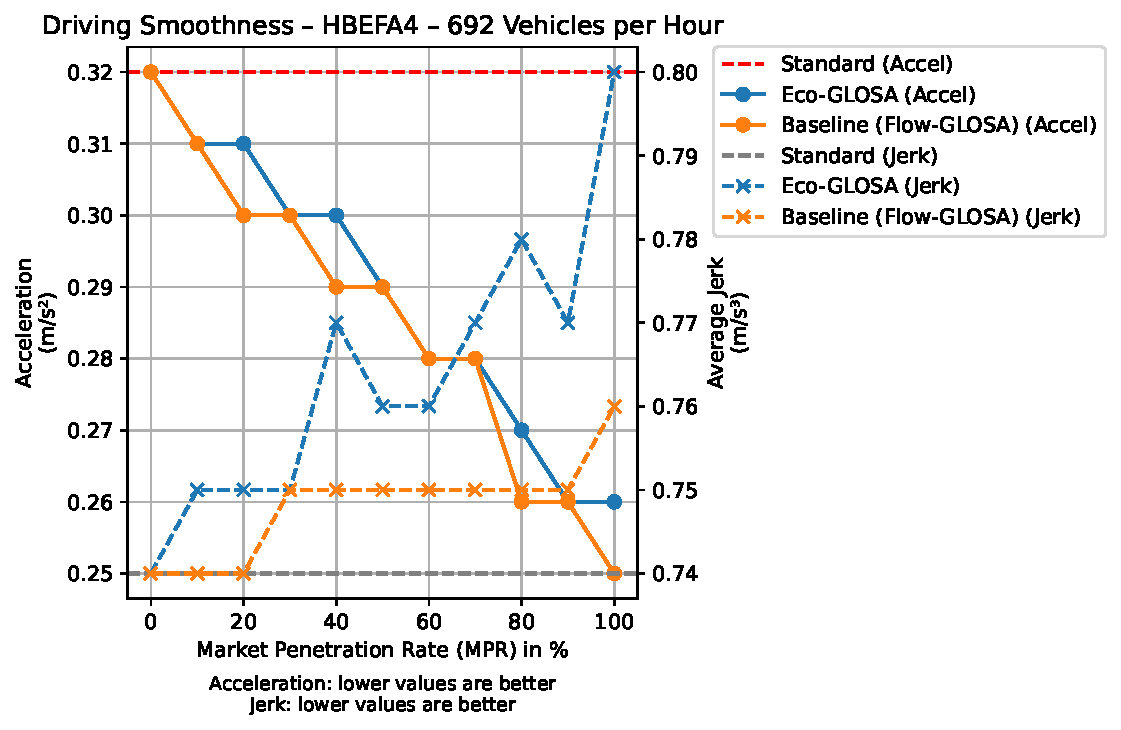
\includegraphics[width=\textwidth]{data/img/DrivingSmoothness/DrivingSmoothness_HBEFA4_Cars692.pdf}
    \caption{Results under the HBEFA4 emission model.}
    \label{fig:Smoothness_HBEFA4_692}
  \end{subfigure}\hfill
  \begin{subfigure}[b]{0.45\textwidth}
    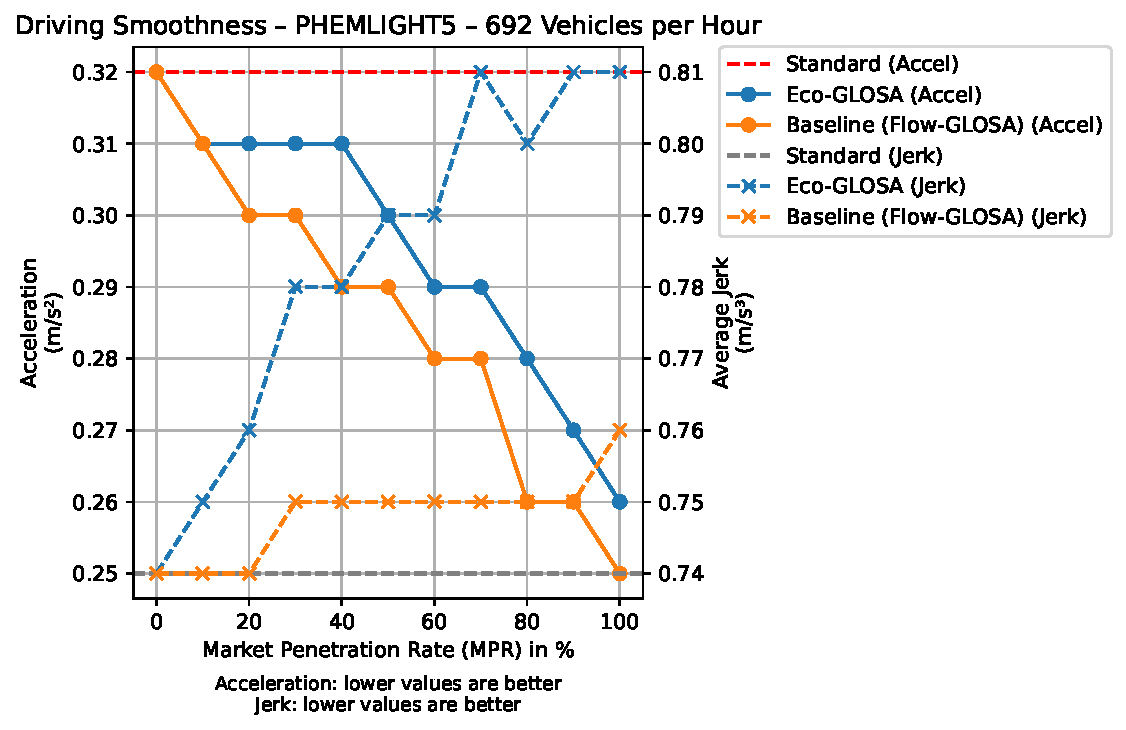
\includegraphics[width=\textwidth]{data/img/DrivingSmoothness/DrivingSmoothness_PHEMLIGHT5_Cars692.pdf}
    \caption{Results under the PHEMlight5 emission model.}
    \label{fig:Smoothness_PHEMlight5_692}
  \end{subfigure}
  \caption[Driving smoothness metrics at $692~\unit{\veh\per\hour}$]{Driving smoothness metrics at a moderate demand of $692~\unit{\veh\per\hour}$. The plots compare average acceleration and jerk for the Standard, \ac{eco-glosa}, and \ac{flow-glosa} controllers.}
  \label{fig:Smoothness_692}
\end{figure}

\paragraph{\ac{eco-glosa} at High Volume ($2769~\unit{\veh\per\hour}$).}
At this demand level, the HBEFA4 model shows fluctuating acceleration values under \ac{eco-glosa}, which rise from the Standard $0.36~\unit{\metre\per\second\squared}$ to $0.41~\unit{\metre\per\second\squared}$ before gradually declining. With the PHEMlight5 model, however, the outcome is more favourable; while not monotonic, the acceleration improves from $0.36~\unit{\metre\per\second\squared}$ to $0.33~\unit{\metre\per\second\squared}$ at full penetration. More significantly, jerk declines to $0.66~\unit{\metre\per\second\cubed}$, a value $13\%$ below the Standard of $0.76~\unit{\metre\per\second\cubed}$ (Figure~\vref{fig:Smoothness_PHEMlight5_2769}). The persistently lower jerk at high \ac{mpr} suggests that once vehicles navigate the initial jam, they maintain smoother trajectories.

\begin{figure}[htb]
  \centering
  \begin{subfigure}[b]{0.45\textwidth}
    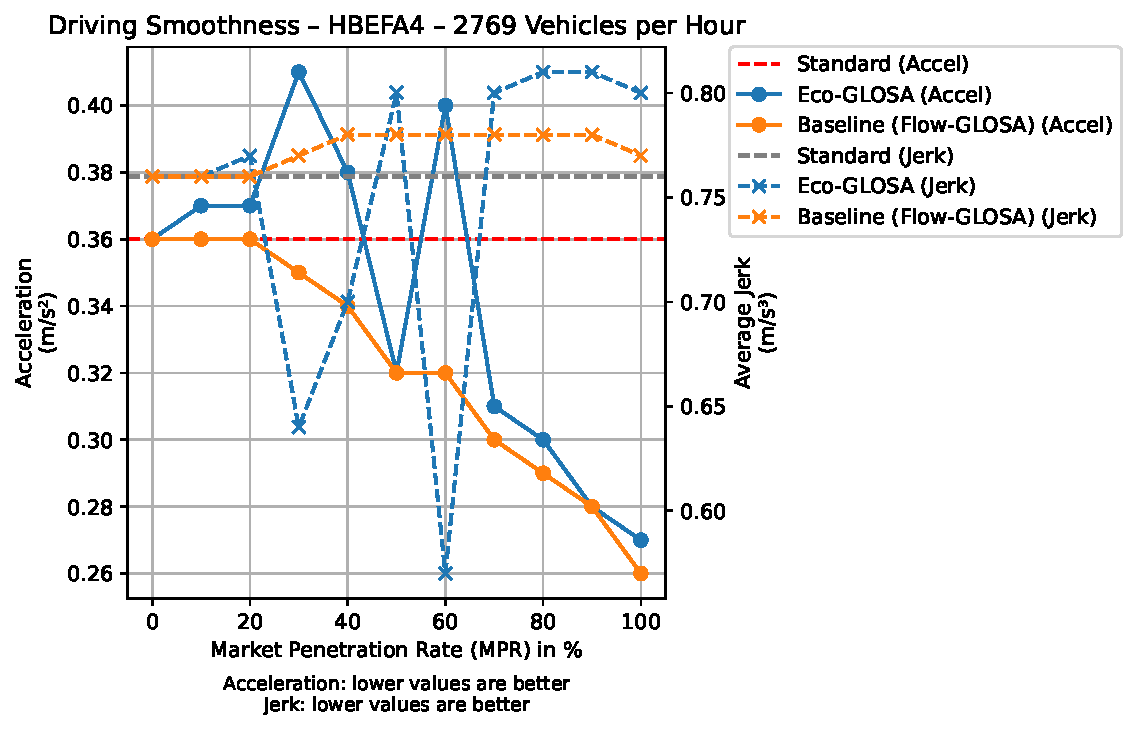
\includegraphics[width=\textwidth]{data/img/DrivingSmoothness/DrivingSmoothness_HBEFA4_Cars2769.pdf}
    \caption{Performance with the HBEFA4 emission model.}
    \label{fig:Smoothness_HBEFA4_2769}
  \end{subfigure}\hfill
  \begin{subfigure}[b]{0.45\textwidth}
    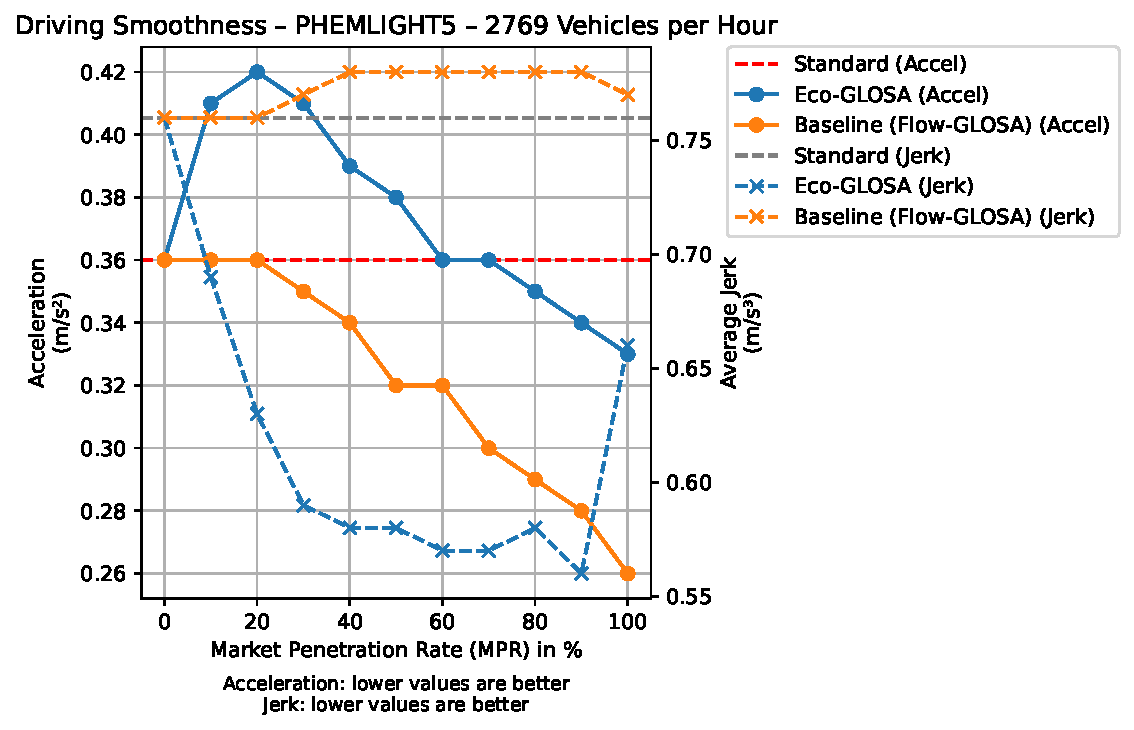
\includegraphics[width=\textwidth]{data/img/DrivingSmoothness/DrivingSmoothness_PHEMLIGHT5_Cars2769.pdf}
    \caption{Performance with the PHEMlight5 emission model.}
    \label{fig:Smoothness_PHEMlight5_2769}
  \end{subfigure}
  \caption[Driving smoothness vs. \ac{mpr} at $2769~\unit{\veh\per\hour}$]{Driving smoothness as a function of \ac{mpr} at the jam threshold of $2769~\unit{\veh\per\hour}$. The plots show the performance of the three controller strategies under two emission models.}
  \label{fig:Smoothness_2769}
\end{figure}

\paragraph{\ac{eco-glosa} at Full Saturation ($3462~\unit{\veh\per\hour}$).}
In the fully saturated regime, both models show clear improvements in smoothness as \ac{mpr} increases. For HBEFA4, acceleration decreases from $0.55$ to $0.38~\unit{\metre\per\second\squared}$ ($31\%$ reduction), and jerk from $0.57$ to $0.51~\unit{\metre\per\second\cubed}$ ($11\%$ reduction) at $100\%$ \ac{mpr}. The PHEMlight5 model shows comparable gains, with acceleration falling to $0.35~\unit{\metre\per\second\squared}$ and jerk to $0.52~\unit{\metre\per\second\cubed}$. However, these smoothness improvements must be interpreted within the context of the traffic jam. As established in Sections~\vref{sec:Results_MeanSpeed} and \vref{sec:Results_Stops}, the controller fails to increase the low average speed or reduce the high stop frequency. Therefore, the data does not indicate a dissolution of the jam. Instead, it suggests that the controller successfully modifies the \enquote{character} of the stop-and-go waves. The aggressive, high-acceleration manoeuvres typical of a congested state are replaced by a smoother, less frantic \enquote{creeping} behaviour. While this change enhances ride comfort, the persistent gridlock confirms that the \ac{eco-glosa} strategy cannot overcome the fundamental capacity limitations at this extreme demand level.

\begin{figure}[htb]
  \centering
  \begin{subfigure}[b]{0.45\textwidth}
    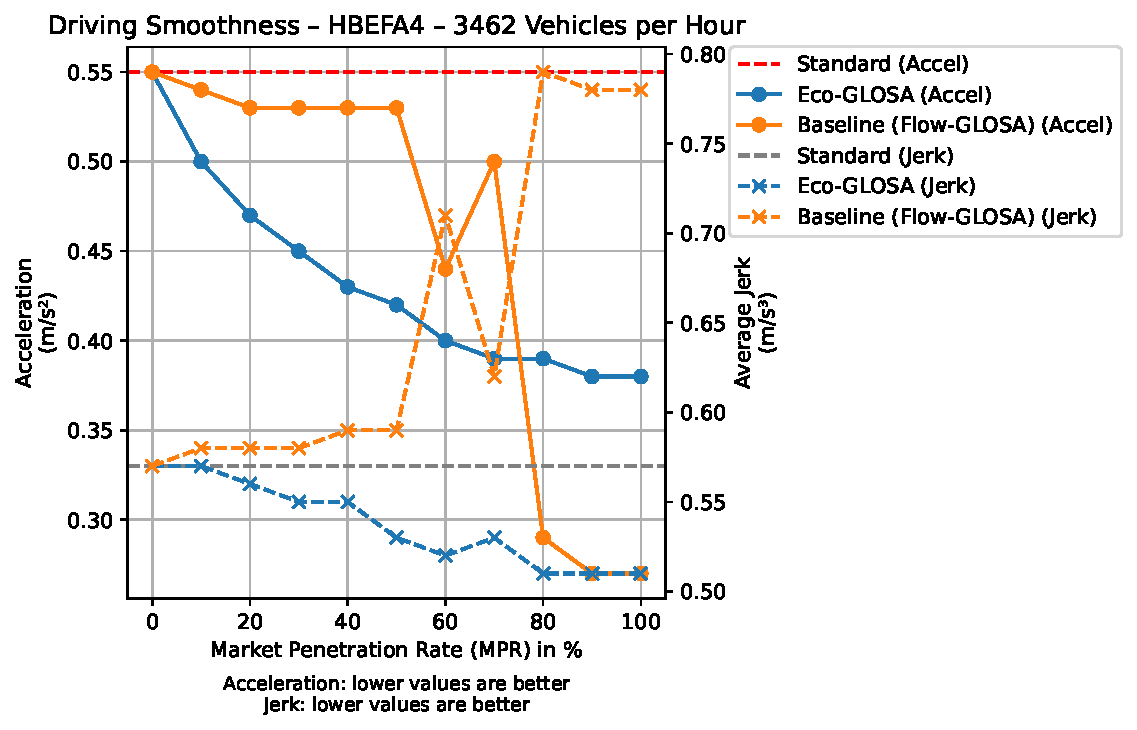
\includegraphics[width=\textwidth]{data/img/DrivingSmoothness/DrivingSmoothness_HBEFA4_Cars3462.pdf}
    \caption{Simulation results using the HBEFA4 model.}
    \label{fig:Smoothness_HBEFA4_3462}
  \end{subfigure}\hfill
  \begin{subfigure}[b]{0.45\textwidth}
    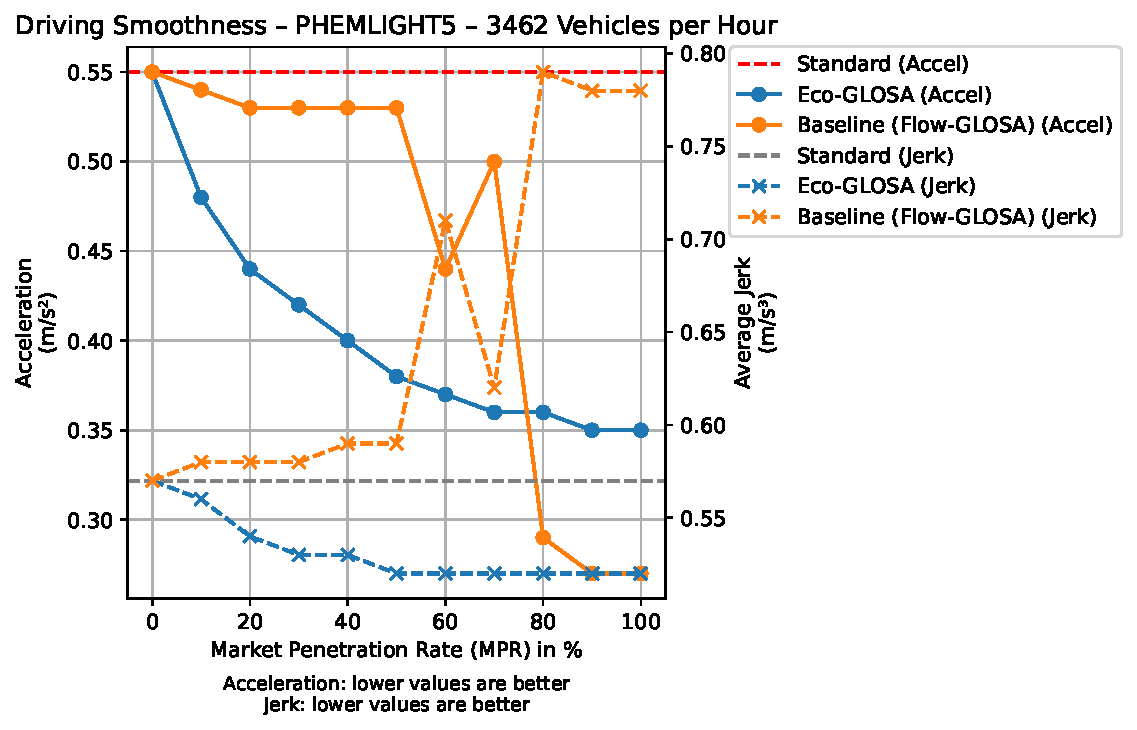
\includegraphics[width=\textwidth]{data/img/DrivingSmoothness/DrivingSmoothness_PHEMLIGHT5_Cars3462.pdf}
    \caption{Simulation results using the PHEMlight5 model.}
    \label{fig:Smoothness_PHEMlight5_3462}
  \end{subfigure}
  \caption[Driving smoothness metrics at $3462~\unit{\veh\per\hour}$]{Driving smoothness metrics in the fully saturated regime ($3462~\unit{\veh\per\hour}$). The plots compare the Standard, \ac{eco-glosa}, and \ac{flow-glosa} controllers.}
  \label{fig:Smoothness_3462}
\end{figure}

\paragraph{\ac{flow-glosa} Comparison.}
The \ac{flow-glosa} controller offers acceleration improvements comparable to \ac{eco-glosa} but generally maintains a more stable and consistently lower jerk profile, except in specific high-saturation scenarios. At low to medium volumes, its application reduces average acceleration by approximately $15\%$ to $20\%$ from the Standard, with only a minimal corresponding increase in average jerk.
\mynewline
The controller's dynamics shift significantly under full saturation ($3462~\unit{\veh\per\hour}$). It exhibits a notable jerk spike from $0.59~\unit{\metre\per\second\cubed}$ to $0.71~\unit{\metre\per\second\cubed}$ at an \ac{mpr} of $60\%$. This transient corresponds precisely to the point where the traffic jam dissolves and vehicles begin to resume free-flow speeds. A second, more pronounced peak appears at $80\%$ \ac{mpr}, which does not stem from an incoming jam but rather from platoon-based micro-adjustments. With such a high share of equipped vehicles, tight clusters form and must continually react to signal timings. Minor mismatches can force abrupt, platoon-wide decelerations and subsequent re-accelerations, which drives the observed increase in average jerk.

\begin{table}[htb]
  \centering
  \caption[Average acceleration and jerk across all volumes and \acp{mpr}]{Driving smoothness, detailed by average acceleration ($\unit{\metre\per\second\squared}$) and jerk ($\unit{\metre\per\second\cubed}$), across all traffic volumes and \acp{mpr}. Results are provided for the Standard, \ac{flow-glosa}, and \ac{eco-glosa} configurations.}
  \label{tab:DrivingSmoothness}
  \resizebox{\textwidth}{!}{%
    \begin{tabular}{l l l *{11}{c}}
      \toprule
      Vehicles & Algorithm & Model       & \textbf{0\% (Standard)} & 10\%        & 20\%        & 30\%        & 40\%        & 50\%        & 60\%        & 70\%        & 80\%        & 90\%        & 100\%       \\
      \midrule
      \textbf{69.0}  & Eco-GLOSA                   & HBEFA4      & \textbf{0.3, 0.74}   & 0.29, 0.75  & 0.31, 0.76  & 0.28, 0.77  & 0.29, 0.77  & 0.29, 0.79  & 0.27, 0.77  & 0.25, 0.81  & 0.28, 0.80  & 0.24, 0.79  & 0.25, 0.81  \\
      \textbf{69.0}  & Baseline (Flow-GLOSA)       & HBEFA4      & \textbf{0.3, 0.74}   & 0.29, 0.76  & 0.31, 0.75  & 0.28, 0.75  & 0.28, 0.75  & 0.29, 0.75  & 0.28, 0.74  & 0.25, 0.75  & 0.27, 0.75  & 0.25, 0.75  & 0.25, 0.77  \\
      \textbf{69.0}  & Eco-GLOSA                   & PHEMlight5  & \textbf{0.3, 0.74}   & 0.29, 0.76  & 0.29, 0.75  & 0.28, 0.76  & 0.27, 0.78  & 0.28, 0.78  & 0.27, 0.80  & 0.25, 0.81  & 0.27, 0.80  & 0.24, 0.79  & 0.23, 0.81  \\
      \textbf{69.0}  & Baseline (Flow-GLOSA)       & PHEMlight5  & \textbf{0.3, 0.74}   & 0.29, 0.76  & 0.31, 0.75  & 0.28, 0.75  & 0.28, 0.75  & 0.29, 0.75  & 0.28, 0.74  & 0.25, 0.75  & 0.27, 0.75  & 0.25, 0.75  & 0.25, 0.77  \\
      \midrule
      \textbf{138.0} & Eco-GLOSA                   & HBEFA4      & \textbf{0.31, 0.73}  & 0.29, 0.74  & 0.30, 0.74  & 0.28, 0.74  & 0.28, 0.77  & 0.27, 0.76  & 0.28, 0.77  & 0.25, 0.77  & 0.27, 0.78  & 0.26, 0.79  & 0.25, 0.78  \\
      \textbf{138.0} & Baseline (Flow-GLOSA)       & HBEFA4      & \textbf{0.31, 0.73}  & 0.29, 0.74  & 0.30, 0.75  & 0.30, 0.73  & 0.28, 0.75  & 0.28, 0.74  & 0.27, 0.75  & 0.26, 0.74  & 0.27, 0.75  & 0.26, 0.74  & 0.25, 0.75  \\
      \textbf{138.0} & Eco-GLOSA                   & PHEMlight5  & \textbf{0.31, 0.73}  & 0.30, 0.73  & 0.29, 0.75  & 0.28, 0.75  & 0.28, 0.77  & 0.26, 0.76  & 0.26, 0.78  & 0.26, 0.77  & 0.26, 0.79  & 0.25, 0.79  & 0.24, 0.79  \\
      \textbf{138.0} & Baseline (Flow-GLOSA)       & PHEMlight5  & \textbf{0.31, 0.73}  & 0.29, 0.74  & 0.30, 0.75  & 0.30, 0.73  & 0.28, 0.75  & 0.28, 0.74  & 0.27, 0.75  & 0.26, 0.74  & 0.27, 0.75  & 0.26, 0.74  & 0.25, 0.75  \\
      \midrule
      \textbf{346.0} & Eco-GLOSA                   & HBEFA4      & \textbf{0.31, 0.74}  & 0.31, 0.75  & 0.31, 0.76  & 0.30, 0.76  & 0.29, 0.76  & 0.29, 0.77  & 0.28, 0.77  & 0.28, 0.77  & 0.27, 0.77  & 0.26, 0.79  & 0.25, 0.80  \\
      \textbf{346.0} & Baseline (Flow-GLOSA)       & HBEFA4      & \textbf{0.31, 0.74}  & 0.31, 0.76  & 0.30, 0.75  & 0.30, 0.76  & 0.29, 0.76  & 0.29, 0.76  & 0.27, 0.75  & 0.28, 0.75  & 0.26, 0.76  & 0.26, 0.76  & 0.24, 0.76  \\
      \textbf{346.0} & Eco-GLOSA                   & PHEMlight5  & \textbf{0.31, 0.74}  & 0.31, 0.75  & 0.31, 0.77  & 0.30, 0.77  & 0.29, 0.77  & 0.28, 0.80  & 0.28, 0.79  & 0.28, 0.78  & 0.26, 0.79  & 0.26, 0.80  & 0.25, 0.82  \\
      \textbf{346.0} & Baseline (Flow-GLOSA)       & PHEMlight5  & \textbf{0.31, 0.74}  & 0.31, 0.76  & 0.30, 0.75  & 0.30, 0.76  & 0.29, 0.76  & 0.29, 0.76  & 0.27, 0.75  & 0.28, 0.75  & 0.26, 0.76  & 0.26, 0.76  & 0.24, 0.76  \\
      \midrule
      \textbf{692.0} & Eco-GLOSA                   & HBEFA4      & \textbf{0.32, 0.74}  & 0.31, 0.75  & 0.31, 0.75  & 0.30, 0.75  & 0.30, 0.77  & 0.29, 0.76  & 0.28, 0.76  & 0.28, 0.77  & 0.27, 0.78  & 0.26, 0.77  & 0.26, 0.80  \\
      \textbf{692.0} & Baseline (Flow-GLOSA)       & HBEFA4      & \textbf{0.32, 0.74}  & 0.31, 0.74  & 0.30, 0.74  & 0.30, 0.75  & 0.29, 0.75  & 0.29, 0.75  & 0.28, 0.75  & 0.28, 0.75  & 0.26, 0.75  & 0.26, 0.75  & 0.25, 0.76  \\
      \textbf{692.0} & Eco-GLOSA                   & PHEMlight5  & \textbf{0.32, 0.74}  & 0.31, 0.75  & 0.31, 0.76  & 0.31, 0.78  & 0.31, 0.78  & 0.30, 0.79  & 0.29, 0.79  & 0.29, 0.81  & 0.28, 0.80  & 0.27, 0.81  & 0.26, 0.81  \\
      \textbf{692.0} & Baseline (Flow-GLOSA)       & PHEMlight5  & \textbf{0.32, 0.74}  & 0.31, 0.74  & 0.30, 0.74  & 0.30, 0.75  & 0.29, 0.75  & 0.29, 0.75  & 0.28, 0.75  & 0.28, 0.75  & 0.26, 0.75  & 0.26, 0.75  & 0.25, 0.76  \\
      \midrule
      \textbf{1385.0}& Eco-GLOSA                   & HBEFA4      & \textbf{0.33, 0.74}  & 0.33, 0.75  & 0.33, 0.76  & 0.32, 0.77  & 0.31, 0.77  & 0.31, 0.77  & 0.30, 0.78  & 0.29, 0.78  & 0.28, 0.78  & 0.27, 0.78  & 0.26, 0.78  \\
      \textbf{1385.0}& Baseline (Flow-GLOSA)       & HBEFA4      & \textbf{0.33, 0.74}  & 0.33, 0.75  & 0.33, 0.75  & 0.32, 0.76  & 0.31, 0.76  & 0.30, 0.76  & 0.29, 0.76  & 0.29, 0.76  & 0.27, 0.76  & 0.27, 0.76  & 0.26, 0.75  \\
      \textbf{1385.0}& Eco-GLOSA                   & PHEMlight5  & \textbf{0.33, 0.74}  & 0.34, 0.77  & 0.34, 0.79  & 0.34, 0.80  & 0.33, 0.81  & 0.32, 0.82  & 0.32, 0.84  & 0.30, 0.83  & 0.29, 0.83  & 0.28, 0.84  & 0.27, 0.83  \\
      \textbf{1385.0}& Baseline (Flow-GLOSA)       & PHEMlight5  & \textbf{0.33, 0.74}  & 0.33, 0.75  & 0.33, 0.75  & 0.32, 0.76  & 0.31, 0.76  & 0.30, 0.76  & 0.29, 0.76  & 0.29, 0.76  & 0.27, 0.76  & 0.27, 0.76  & 0.26, 0.75  \\
      \midrule
      \textbf{2077.0}& Eco-GLOSA                   & HBEFA4      & \textbf{0.34, 0.75}  & 0.34, 0.75  & 0.35, 0.76  & 0.34, 0.77  & 0.33, 0.78  & 0.32, 0.78  & 0.31, 0.78  & 0.30, 0.79  & 0.29, 0.79  & 0.28, 0.78  & 0.27, 0.78  \\
      \textbf{2077.0}& Baseline (Flow-GLOSA)       & HBEFA4      & \textbf{0.34, 0.75}  & 0.34, 0.76  & 0.34, 0.76  & 0.33, 0.76  & 0.32, 0.77  & 0.32, 0.77  & 0.30, 0.77  & 0.29, 0.77  & 0.28, 0.76  & 0.26, 0.76  & 0.26, 0.76  \\
      \textbf{2077.0}& Eco-GLOSA                   & PHEMlight5  & \textbf{0.34, 0.75}  & 0.36, 0.78  & 0.35, 0.80  & 0.35, 0.82  & 0.34, 0.84  & 0.32, 0.84  & 0.31, 0.85  & 0.31, 0.87  & 0.29, 0.86  & 0.28, 0.86  & 0.27, 0.87  \\
      \textbf{2077.0}& Baseline (Flow-GLOSA)       & PHEMlight5  & \textbf{0.34, 0.75}  & 0.34, 0.76  & 0.34, 0.76  & 0.33, 0.76  & 0.32, 0.77  & 0.32, 0.77  & 0.30, 0.77  & 0.29, 0.77  & 0.28, 0.76  & 0.26, 0.76  & 0.26, 0.76  \\
      \midrule
      \textbf{2769.0}& Eco-GLOSA                   & HBEFA4      & \textbf{0.36, 0.76}  & 0.37, 0.76  & 0.37, 0.77  & 0.41, 0.64  & 0.38, 0.70  & 0.32, 0.80  & 0.40, 0.57  & 0.31, 0.80  & 0.30, 0.81  & 0.28, 0.81  & 0.27, 0.80  \\
      \textbf{2769.0}& Baseline (Flow-GLOSA)       & HBEFA4      & \textbf{0.36, 0.76}  & 0.36, 0.76  & 0.36, 0.76  & 0.35, 0.77  & 0.34, 0.78  & 0.32, 0.78  & 0.32, 0.78  & 0.30, 0.78  & 0.29, 0.78  & 0.28, 0.78  & 0.26, 0.77  \\
      \textbf{2769.0}& Eco-GLOSA                   & PHEMlight5  & \textbf{0.36, 0.76}  & 0.41, 0.69  & 0.42, 0.63  & 0.41, 0.59  & 0.39, 0.58  & 0.38, 0.58  & 0.36, 0.57  & 0.36, 0.57  & 0.35, 0.58  & 0.34, 0.56  & 0.33, 0.66  \\
      \textbf{2769.0}& Baseline (Flow-GLOSA)       & PHEMlight5  & \textbf{0.36, 0.76}  & 0.36, 0.76  & 0.36, 0.76  & 0.35, 0.77  & 0.34, 0.78  & 0.32, 0.78  & 0.32, 0.78  & 0.30, 0.78  & 0.29, 0.78  & 0.28, 0.78  & 0.26, 0.77  \\
      \midrule
      \textbf{3462.0} & \textbf{Eco-GLOSA} & \textbf{HBEFA4} & \textbf{0.55, 0.57} & \textbf{0.50, 0.57} & \textbf{0.47, 0.56} & \textbf{0.45, 0.55} & \textbf{0.43, 0.55} & \textbf{0.42, 0.53} & \textbf{0.40, 0.52} & \textbf{0.39, 0.53} & \textbf{0.39, 0.51} & \textbf{0.38, 0.51} & \textbf{0.38, 0.51} \\
      \textbf{3462.0}& Baseline (Flow-GLOSA)       & HBEFA4      & \textbf{0.55, 0.57}  & 0.54, 0.58  & 0.53, 0.58  & 0.53, 0.58  & 0.53, 0.59  & 0.53, 0.59  & 0.44, 0.71  & 0.50, 0.62  & \textbf{0.29, 0.79}  & \textbf{0.27, 0.78}  & \textbf{0.27, 0.78}  \\
      \textbf{3462.0} & \textbf{Eco-GLOSA} & \textbf{PHEMlight5} & \textbf{0.55, 0.57} & \textbf{0.48, 0.56} & \textbf{0.44, 0.54} & \textbf{0.42, 0.53} & \textbf{0.40, 0.53} & \textbf{0.38, 0.52} & \textbf{0.37, 0.52} & \textbf{0.36, 0.52} & \textbf{0.36, 0.52} & \textbf{0.35, 0.52} & \textbf{0.35, 0.52} \\
      \textbf{3462.0}& Baseline (Flow-GLOSA)       & PHEMlight5  & \textbf{0.55, 0.57}  & 0.54, 0.58  & 0.53, 0.58  & 0.53, 0.58  & 0.53, 0.59  & 0.53, 0.59  & 0.44, 0.71  & 0.50, 0.62  & \textbf{0.29, 0.79}  & \textbf{0.27, 0.78}  & \textbf{0.27, 0.78}  \\
      \bottomrule
    \end{tabular}%
  }
\end{table}
